\documentclass[11pt]{article}
\usepackage[a4paper,margin=2.3cm]{geometry}
\usepackage{amsmath,amssymb}
\usepackage{booktabs,array}
\usepackage{enumitem}
\usepackage[dvipsnames]{xcolor}
\usepackage[most]{tcolorbox}
\usepackage{tikz}
\usetikzlibrary{positioning,decorations.pathreplacing,arrows.meta,shapes.geometric}
\usepackage{microtype}
\usepackage[colorlinks=true,linkcolor=NavyBlue,urlcolor=NavyBlue]{hyperref}

\newtcolorbox{keybox}[1][]{colback=Gray!6,colframe=Gray!55,boxrule=0.5pt,arc=2pt,
  left=6pt,right=6pt,top=5pt,bottom=5pt,#1}
\newtcolorbox{warnbox}[1][]{colback=BrickRed!5,colframe=BrickRed!60,boxrule=0.6pt,arc=2pt,
  left=6pt,right=6pt,top=5pt,bottom=5pt,#1}

\title{\textbf{How the Antennas Are Arranged in Each Configuration}\\[3pt]
\large ULA, USA, ECA --- and why ``local'' and ``CAPE'' are \emph{not} new arrangements}
\author{Explanatory note (simple English)}
\date{\today}

% draw one antenna row at true relative scale (index unit = lambda/2)
\newcommand{\antrow}[3]{% #1=color #2=yscale-ignore #3=comma list
  \begin{scope}[xscale=0.075]
  \foreach \x in {#3} {\fill[#1] (\x,0) circle (1.1pt);}
  \end{scope}}

\begin{document}
\maketitle

\begin{keybox}
\textbf{The most important thing first.} In your study there are really only
\emph{three} physical antenna arrangements: the \textbf{dense ULA}, the \textbf{uniform sparse
(USA)}, and the \textbf{ECA} (and a smaller ECA used as a control). The names you see in the
figures --- ``ULA + local'', ``ULA + CAPE'', ``ECA + local'', ``ECA + CAPE'' --- are
\textbf{not four different arrangements}. They are two arrangements (ULA and ECA), each used with
two different \emph{processing methods} (``local'' or ``CAPE''). \emph{The antennas do not move
when you switch from local to CAPE.}
\end{keybox}

%====================================================================
\section{Two separate things: arrangement vs.\ processing}

\begin{center}
\renewcommand{\arraystretch}{1.25}
\begin{tabular}{@{}p{4.6cm}p{10.0cm}@{}}
\toprule
\textbf{Antenna arrangement} (hardware: where the antennas sit) &
\textbf{Processing method} (software: what we do with the received signals)\\
\midrule
ULA --- dense, equal spacing & \textbf{local} --- each AP estimates its own channel by itself\\
USA --- sparse, equal spacing & \textbf{CAPE} --- the APs cooperate to find the user's position first\\
ECA --- sparse, \emph{unequal} spacing & \\
\bottomrule
\end{tabular}
\end{center}

A ``scheme'' in your figures is one arrangement \emph{plus} one processing method:

\begin{center}
\renewcommand{\arraystretch}{1.25}
\begin{tabular}{@{}lll l@{}}
\toprule
Scheme in the figures & Antennas (hardware) & Processing (software) & Role\\
\midrule
ULA + local        & dense ULA (64) & local & your original baseline\\
ECA + local        & ECA (63)       & local & plain sparse array (Code C)\\
ULA + CAPE          & dense ULA (64) & CAPE  & control / ablation\\
ECA + CAPE (proposed) & ECA (63)     & CAPE  & \textbf{the proposed system}\\
\bottomrule
\end{tabular}
\end{center}

\begin{keybox}
Read it as ``\textbf{arrangement} + \textbf{processing}''. ``ULA + local'' and ``ULA + CAPE'' are
the \emph{same antennas}, processed two different ways. ``ECA + local'' and ``ECA + CAPE'' are the
\emph{same antennas}, processed two different ways.
\end{keybox}

%====================================================================
\section{The antenna arrangements (hardware)}

All arrays use about the same number of antennas ($\approx 64$). The spacing unit below is
$d_0=\lambda/2 = 5$\,cm (half a wavelength at 3\,GHz). Each arrangement just decides \emph{where}
the antennas sit on the line.

\subsection{Dense ULA --- equal small spacing}
Every antenna is exactly one step ($d_0$) from the next. 64 antennas, total length 3.15\,m.
Short array $\Rightarrow$ poor ability to focus in distance, but no ghost beams.
\begin{center}
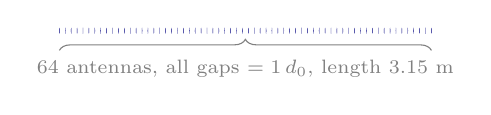
\begin{tikzpicture}
\antrow{NavyBlue}{0}{-31.5,-30.5,-29.5,-28.5,-27.5,-26.5,-25.5,-24.5,-23.5,-22.5,-21.5,-20.5,-19.5,-18.5,-17.5,-16.5,-15.5,-14.5,-13.5,-12.5,-11.5,-10.5,-9.5,-8.5,-7.5,-6.5,-5.5,-4.5,-3.5,-2.5,-1.5,-0.5,0.5,1.5,2.5,3.5,4.5,5.5,6.5,7.5,8.5,9.5,10.5,11.5,12.5,13.5,14.5,15.5,16.5,17.5,18.5,19.5,20.5,21.5,22.5,23.5,24.5,25.5,26.5,27.5,28.5,29.5,30.5,31.5}
\draw[decorate,decoration={brace,amplitude=4pt},Gray] (-31.5*0.075,-0.25) -- (31.5*0.075,-0.25)
  node[midway,below,font=\scriptsize]{64 antennas, all gaps $=1\,d_0$, length 3.15 m};
\end{tikzpicture}
\end{center}

\subsection{Uniform sparse (USA) --- equal \emph{large} spacing}
Same 64 antennas, but every gap is two steps ($2d_0=\lambda$). The array is now twice as long
(6.30\,m), so it is sharper --- \emph{but} equal large spacing creates exact copies of the beam at
other angles (grating lobes / ghost beams). This is why USA is not used in the end.
\begin{center}
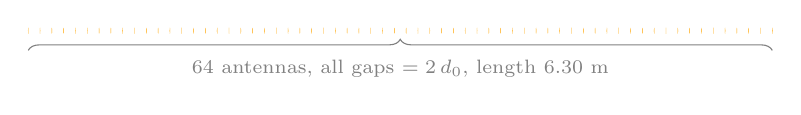
\begin{tikzpicture}
\antrow{Orange}{0}{-63,-61,-59,-57,-55,-53,-51,-49,-47,-45,-43,-41,-39,-37,-35,-33,-31,-29,-27,-25,-23,-21,-19,-17,-15,-13,-11,-9,-7,-5,-3,-1,1,3,5,7,9,11,13,15,17,19,21,23,25,27,29,31,33,35,37,39,41,43,45,47,49,51,53,55,57,59,61,63}
\draw[decorate,decoration={brace,amplitude=4pt},Gray] (-63*0.075,-0.25) -- (63*0.075,-0.25)
  node[midway,below,font=\scriptsize]{64 antennas, all gaps $=2\,d_0$, length 6.30 m};
\end{tikzpicture}
\end{center}

\subsection{ECA --- sparse with \emph{unequal} spacing (the proposed array)}
63 antennas placed at \emph{uneven} gaps, so the array is the widest (7.60\,m) and sharpest, yet
the uneven gaps stop the ghost copies from lining up --- no strong ghost beams.
\begin{center}
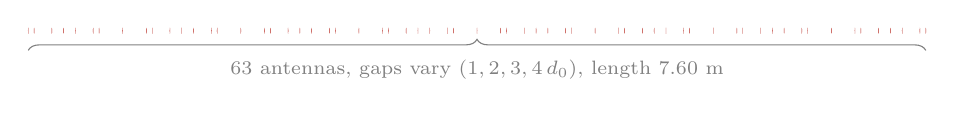
\begin{tikzpicture}
\antrow{BrickRed}{0}{-76,-75,-72,-70,-68,-65,-64,-60,-56,-55,-52,-50,-48,-45,-44,-40,-36,-35,-32,-30,-28,-25,-24,-20,-16,-15,-12,-10,-8,-5,-4,0,4,5,8,10,12,15,16,20,24,25,28,30,32,35,36,40,44,45,48,50,52,55,56,60,64,65,68,70,72,75,76}
\draw[decorate,decoration={brace,amplitude=4pt},Gray] (-76*0.075,-0.25) -- (76*0.075,-0.25)
  node[midway,below,font=\scriptsize]{63 antennas, gaps vary ($1,2,3,4\,d_0$), length 7.60 m};
\end{tikzpicture}
\end{center}

\paragraph{How the ECA gaps are built (the co-prime recipe).}
Take two numbers with no common factor: $M=5$ and $N=4$. One ``block'' is made of two rulers that
share their first antenna:
\begin{itemize}[leftmargin=1.5em,itemsep=1pt]
\item a 5-antenna ruler with gap $4\,d_0$: positions $0,4,8,12,16$;
\item a 4-antenna ruler with gap $5\,d_0$: positions $0,5,10,15$.
\end{itemize}
Merging them (position $0$ is shared) gives 8 antennas at $\{0,4,5,8,10,12,15,16\}$. This block is
repeated 8 times (period $20\,d_0$) and mirrored about the centre, giving 63 antennas. The gap
pattern that repeats along the array is
\[
\dots,\;1,\;3,\;2,\;2,\;3,\;1,\;4,\;4,\;\dots\quad(\text{in units of }d_0).
\]
\begin{center}
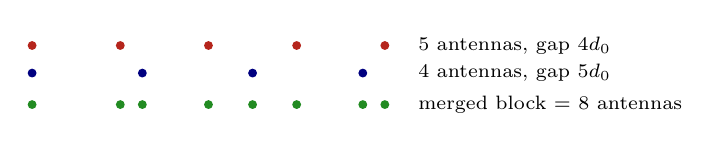
\begin{tikzpicture}[scale=1.0]
\foreach \x in {0,4,8,12,16} {\fill[BrickRed] (\x*0.28,0.35) circle (1.6pt);}
\node[font=\scriptsize,anchor=west] at (16*0.28+0.3,0.35) {5 antennas, gap $4d_0$};
\foreach \x in {0,5,10,15} {\fill[NavyBlue] (\x*0.28,0) circle (1.6pt);}
\node[font=\scriptsize,anchor=west] at (16*0.28+0.3,0) {4 antennas, gap $5d_0$};
\foreach \x in {0,4,5,8,10,12,15,16} {\fill[ForestGreen] (\x*0.28,-0.4) circle (1.6pt);}
\node[font=\scriptsize,anchor=west] at (16*0.28+0.3,-0.4) {merged block = 8 antennas};
\end{tikzpicture}
\end{center}

\subsection{ECA same-aperture (the small control)}
The same ECA recipe but with only 4 blocks instead of 8: 31 antennas over 3.60\,m (about the
dense ULA's length). It is in the study only to separate ``more aperture'' from ``sparser
spacing''; it is not the proposed array.

\begin{center}
\renewcommand{\arraystretch}{1.22}
\begin{tabular}{@{}lcccp{4.2cm}@{}}
\toprule
Arrangement & Antennas & Gaps & Length & Ghost beams\\
\midrule
Dense ULA           & 64 & all $1\,d_0$      & 3.15 m & none\\
Uniform sparse USA  & 64 & all $2\,d_0$      & 6.30 m & \textbf{strong}\\
\textbf{ECA (proposed)} & 63 & $1,2,3,4\,d_0$ & \textbf{7.60 m} & none (suppressed)\\
ECA same-aperture   & 31 & $1,2,3,4\,d_0$   & 3.60 m & none (control)\\
\bottomrule
\end{tabular}
\end{center}

%====================================================================
\section{The processing methods (software) --- same antennas}

These do \emph{not} change the antenna positions. They change only how the central processor turns
the received pilot signals into a channel estimate.

\begin{description}[leftmargin=0pt,itemsep=4pt]
\item[\textbf{``local'' estimation.}] Each AP looks at its own antennas only and guesses the
  user's channel by itself. Fast and simple. Problem on a sparse array: the AP sees several
  ``maybe'' spots (ambiguity) and sometimes picks the wrong one, so the estimate is noisier. This
  is the old method (your baseline and Code C).
\item[\textbf{``CAPE'' estimation (proposed).}] The APs \emph{cooperate}. A user has only one true
  location; the strongest APs propose candidate positions, the central processor keeps the one
  position that all of them agree on (the false spots of one AP are killed by the others), and
  then every AP builds its channel from that single agreed position. Same antennas, smarter use of
  them.
\end{description}

\begin{center}
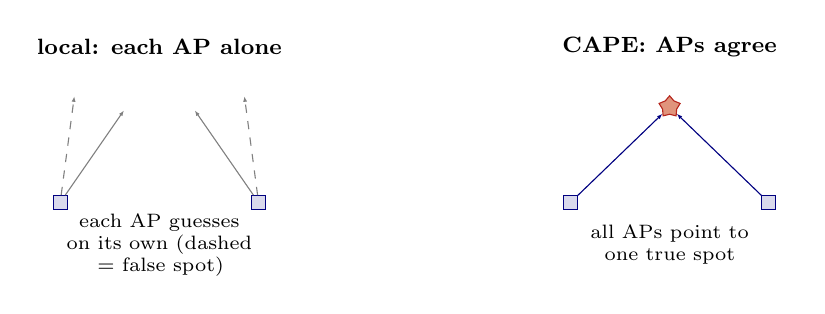
\begin{tikzpicture}[scale=0.9,
  ap/.style={rectangle,draw=NavyBlue,fill=NavyBlue!15,minimum size=5pt,inner sep=2pt}]
% local
\begin{scope}
  \node[font=\footnotesize\bfseries] at (1.4,2.2) {local: each AP alone};
  \node[ap] (a) at (0,0) {}; \node[ap] (b) at (2.8,0) {};
  \draw[Gray,-{Latex[length=2pt]}] (a) -- (0.9,1.3); \draw[Gray,dashed,-{Latex[length=2pt]}] (a) -- (0.2,1.5);
  \draw[Gray,-{Latex[length=2pt]}] (b) -- (1.9,1.3); \draw[Gray,dashed,-{Latex[length=2pt]}] (b) -- (2.6,1.5);
  \node[font=\scriptsize,text width=3cm,align=center] at (1.4,-0.6){each AP guesses on its own (dashed = false spot)};
\end{scope}
% cape
\begin{scope}[xshift=7.2cm]
  \node[font=\footnotesize\bfseries] at (1.4,2.2) {CAPE: APs agree};
  \node[ap] (a2) at (0,0) {}; \node[ap] (b2) at (2.8,0) {};
  \node[star,star points=5,draw=BrickRed,fill=BrickRed!40,minimum size=8pt,inner sep=0.4pt] (u2) at (1.4,1.35) {};
  \draw[NavyBlue,-{Latex[length=2pt]}] (a2) -- (u2); \draw[NavyBlue,-{Latex[length=2pt]}] (b2) -- (u2);
  \node[font=\scriptsize,text width=3cm,align=center] at (1.4,-0.6){all APs point to one true spot};
\end{scope}
\end{tikzpicture}
\end{center}

\begin{warnbox}
\textbf{Why ULA + CAPE is in the study but is a bad idea.} CAPE needs a sharp position fix, which
only a \emph{wide} array gives. The dense ULA is short, so its position fix is poor; forcing CAPE
on it makes things worse (its curves floor out). So CAPE belongs with the \emph{sparse} array.
``ULA + CAPE'' is kept only to prove this point --- that the array and the processing must go
together. The winning pair is \textbf{ECA + CAPE}.
\end{warnbox}

%====================================================================
\section{One-page summary}

\begin{keybox}
\begin{itemize}[leftmargin=1.3em,itemsep=2pt]
\item \textbf{ULA}: 64 antennas, equal $\lambda/2$ gaps, short (3.15 m). Simple, low resolution.
\item \textbf{USA}: 64 antennas, equal $\lambda$ gaps, long (6.30 m). Sharp but has ghost beams.
\item \textbf{ECA}: 63 antennas, \emph{unequal} gaps ($1$--$4\,d_0$), longest (7.60 m). Sharp,
      no ghosts --- the proposed array (from the 2025 ECA paper).
\item \textbf{``local'' and ``CAPE'' are processing, not arrangements.} The antennas are identical;
      only the way the signals are combined changes.
\item \textbf{ECA + CAPE} = the proposed system: the widest, sharpest array, made reliable by
      letting the APs agree on the user's position.
\end{itemize}
\end{keybox}

\end{document}
